

\documentclass{article}

\usepackage{multicol}
\setlength{\columnsep}{1.2cm}
\usepackage{pgfplots}
\pgfplotsset{compat = newest}

\begin{document}

\section{Intro to Functions}

\subsection{Transformations}

\[ y = af(k(x-d))+c \]

\noindent
Where:
\begin{itemize}
	\item a and c affect the y-coordinate
	\item k and d affect the x-coordinate
\end{itemize}

\subsubsection*{Functions}

\begin{multicols}{2}
\noindent
Quadratic Function\\
$y = x^{2}$\\
$y = a(k(x-d))^{2}+c$\\\\
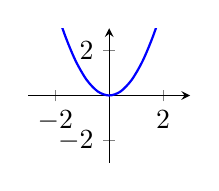
\begin{tikzpicture}
	\begin{axis}[scale = 0.3, axis lines = center, xmin=-3, xmax=3, ymin=-3, ymax=3]
		\addplot[blue,smooth, thick] {x^2};
	\end{axis}
\end{tikzpicture}\\

\noindent
Root Function\\
$y = \sqrt{x}$\\
$y = a\sqrt{k(x-d)}+c$\\\\
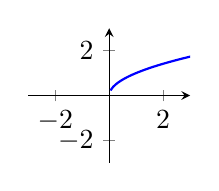
\begin{tikzpicture}
	\begin{axis}[ axis lines = center, xmin=-3, xmax=3, ymin=-3, ymax=3, scale = 0.3, samples=100]
		\addplot[blue, smooth, thick, unbounded coords = jump] {sqrt(x)};
	\end{axis}
\end{tikzpicture}\\

\noindent
Cubic Function\\
$y = x^{3}$\\
$y = a(k(x-d))^{3}+c$\\\\
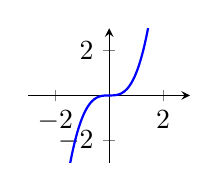
\begin{tikzpicture}
	\begin{axis}[ axis lines = center, xmin=-3, xmax=3, ymin=-3, ymax=3, scale = 0.3, samples=100]
		\addplot[blue, smooth, thick, unbounded coords = jump] {x^3};
	\end{axis}
\end{tikzpicture}\\

\noindent
Absolute Value Function\\
$y = |x|$\\
$y = a|k(x-d)|+c$\\\\
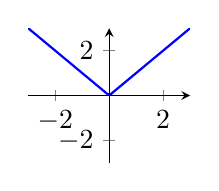
\begin{tikzpicture}
	\begin{axis}[ axis lines = center, xmin=-3, xmax=3, ymin=-3, ymax=3, scale = 0.3, samples=100]
		\addplot[blue, smooth, thick, unbounded coords = jump] {abs(x)};
	\end{axis}
\end{tikzpicture}\\

\noindent
Reciprocal Function\\
$y = \frac{1}{x}$\\
$y = \frac{a}{k(x-d)}+c$\\\\
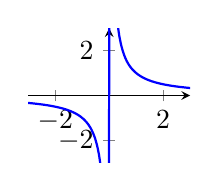
\begin{tikzpicture}
	\begin{axis}[ axis lines = center, xmin=-3, xmax=3, ymin=-3, ymax=3, scale = 0.3, samples=100]
		\addplot[blue, smooth, thick, unbounded coords = jump] {1/x};
	\end{axis}
\end{tikzpicture}\\

\noindent
Exponential Function\\
$y = 2^{x}$\\
$y = a2^{k(x-d)}+c$\\\\
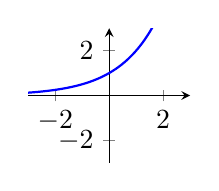
\begin{tikzpicture}
	\begin{axis}[ axis lines = center, xmin=-3, xmax=3, ymin=-3, ymax=3, scale = 0.3, samples=100]
		\addplot[blue, smooth, thick, unbounded coords = jump] {2^x};
	\end{axis}
\end{tikzpicture}\\

\end{multicols}

\newpage
\noindent
Effects of Letters\\

\begin{multicols}{2}

\noindent
a:

\begin{verbatim}
0 < |a| < 1
\end{verbatim}

\noindent
Vertical compression by a factor of $|a|$\\
Multiply y values by $|a|$\\\\

\begin{verbatim}
|a| > 1
\end{verbatim}

\noindent
Vertical stretch by a factor of $|a|$\\
Multiply y values by $|a|$\\\\

\begin{verbatim}
a < 0
\end{verbatim}

\noindent
Reflection over the x-axis\\
Multiply y values by -1\\

\columnbreak

\noindent
k:

\begin{verbatim}
0 < |k| < 1
\end{verbatim}

\noindent
Horizontal stretch by a factor of $\frac{1}{|k|}$\\
Multiply x values by $\frac{1}{|k|}$\\\\

\begin{verbatim}
|k| > 1
\end{verbatim}

\noindent
Horizontal compression by $\frac{1}{|k|}$\\
Multiply x values by $\frac{1}{|k|}$\\\\

\begin{verbatim}
k<0
\end{verbatim}

\noindent
Reflection over the y-axis\\
Multiply x values by -1\\\\

\end{multicols}

\begin{multicols}{2}
\noindent
c:

\begin{verbatim}
c > 0
\end{verbatim}

\noindent
Shift up c units\\
Add c to y values\\\\

\begin{verbatim}
c < 0
\end{verbatim}

\noindent
Shift down c units\\
Add c to y values\\\\

\columnbreak
\noindent
d:

\begin{verbatim}
d > 0
\end{verbatim}

\noindent
Shift right d units\\
Add d to x values\\\\

\begin{verbatim}
d < 0
\end{verbatim}

\noindent
Shift left d units\\
Add d to x values \\

\end{multicols}

\noindent
Notes:\\
- k must be factored out in order to determine the value of d\\
- The order to complete transformations is:
\begin{verbatim}
   1) Stretch/Compress
   2) Reflect
   3) Shift
\end{verbatim}

\end{document}